\documentclass{standalone}

\usepackage{tikz}

\begin{document}
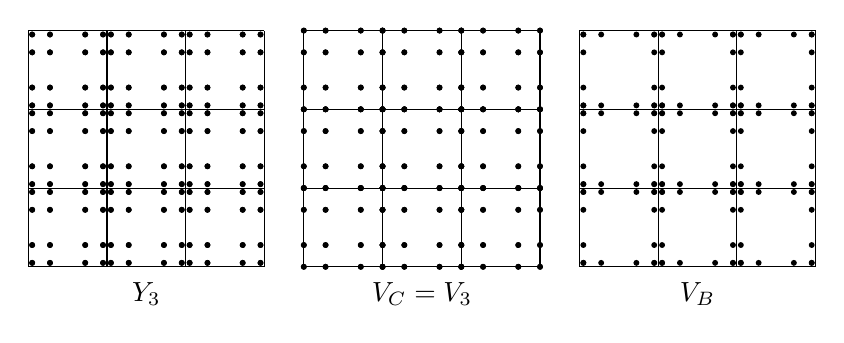
\begin{tikzpicture}
	\def\gap{.05}
	\def\rad{.85pt}
	\def\labh{-.35}
	\draw (0,0) grid (3,3); 
	\foreach \i in {0,...,2}{
		\foreach \j in {0,...,2}{
			\begin{scope}[shift={(\i,\j)}]
				\foreach \x in {\gap,2.76393202e-01, 7.23606798e-01,1-\gap}{
					\foreach \y in {\gap,2.76393202e-01, 7.23606798e-01,1-\gap}{
						\filldraw (\x,\y) circle[radius=\rad];
						\filldraw (\y,\x) circle[radius=\rad]; 				
					}
				}
			\end{scope}
		}
	}
	\node at (1.5,\labh) {$Y_3$}; 

	\begin{scope}[xshift=3.5cm]
		\draw (0,0) grid (3,3); 
		\foreach \i in {0,...,2}{
			\foreach \j in {0,...,2}{
				\begin{scope}[shift={(\i,\j)}]
					\foreach \x in {0,2.76393202e-01, 7.23606798e-01,1}{
						\foreach \y in {0,2.76393202e-01, 7.23606798e-01,1}{
							\filldraw (\x,\y) circle[radius=\rad];
							\filldraw (\y,\x) circle[radius=\rad]; 				
						}
					}
				\end{scope}
			}
		}
		\node at (1.5, \labh) {$V_C = V_3$}; 
	\end{scope}

	\begin{scope}[xshift=7cm]
		\draw (0,0) grid (3,3); 
		\foreach \i in {0,...,2}{
			\foreach \j in {0,...,2}{
				\begin{scope}[shift={(\i,\j)}]
					\foreach \x in {\gap,2.76393202e-01, 7.23606798e-01,1-\gap}{
						\foreach \y in {\gap,1-\gap}{
							\filldraw (\x,\y) circle[radius=\rad];
							\filldraw (\y,\x) circle[radius=\rad]; 				
						}
					}
					% \foreach \x in {2.76393202e-01, 7.23606798e-01}{
					% 	\foreach \y in {2.76393202e-01, 7.23606798e-01}{
					% 		\filldraw[black!10] (\x,\y) circle[radius=\rad];
					% 	} 				
					% }
				\end{scope}
			}
		}
		\node at (1.5, \labh) {$V_B$}; 
	\end{scope}
\end{tikzpicture}
\end{document}